\section{Tutte's Sequential Algorithm}

To obtain the graph resulting from the Tutte theorem, an algorithm is
needed. In this section, a sequential algorithm is described. This
algorithm is an iterative solution. To compute a solution, a set of nodes
 making up a convex polygon must be decided. Let $P$ be this set of nodes. Let
$G_k$ be the graph generated at the step $k$.
\\

To obtain the graph of the next step, all the nodes of the interior of the
convex polygon $P$ will be visited. For each node visited, the barycentric
coordinates of its neighbourhood are computed. Then these coordinates are used
to update the position of the current node. Once each node has been visited,
the computation of the graph $G_{k+1}$ is completed.
\\
In this project, the stop condition used for this algorithm is an epsilon
between the relative positions of the node of the graph $G_k$ and
$G_{k+1}$. For all nodes of the graph, if the length of each movement is
inferior to a given epsilon, the graph $G_{k+1}$ is the solution.
\\

The figure \ref{transition} gives an exemple of the mouvement of one node
during one step.
\begin{figure}[!h]
\centering
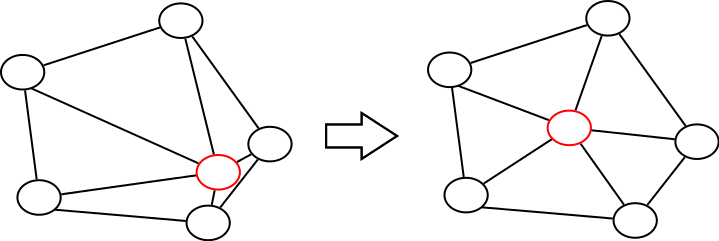
\includegraphics[scale=0.5]{img/transition.png}
\caption{barycenter computation of the red node}
\label{transition}
\end{figure}

This gives a synthetic view of this algorithm : 
\begin{verbatim}
G = {V,E}
P = set of nodes constituent a convex polygon
procedure tutte(G, P, epsilon)
  epsilon_current = 0
  for each node of (V \ convex polygon)
    barycenter = barycenter of neighboring nodes
    epsilon_current = max(epsilon_current, distance(node, barycenter))
    node = barycenter
  if (epsilon_current < epsilon)
    exit()
  tutte(G, P, epsilon)
\end{verbatim}

From the complexity point of view, during one iteration all the nodes of
the set $V$ - $convex~polygon$ are visited. For each node, all its
neighbourhood is visited. Let $mean\_d$ be the average degree of this planar
graph. So the compexity of an iteration is $\mathit{O(n \times mean\_d)}$
with $n = |V|$.

% Le but ici est d'exposé la méthode algorithmique qui découle de l'algorithme de Tutte et  de prouver que cette méthode converge (retrouver l'article qui en parle)
